% Provenance (never printed): cycle 4 SVT, "La planete Terre, l'environnement":
% glaciers and their landforms, the cryosphere, the glaciations told; see
% sources/book1/PROVENANCE.md. Book 1, grade 8, chapter 5.
% Vocabulary guard: owns glacier; ice sheet + ice shelf + iceberg (one
% definition); sea ice; permafrost; U-shaped valley + moraine (one
% definition); ice age. "Glacial period", "interglacial" and "glacial cycle"
% belong to Book 2 g12 past-climates: here "the ice ages and the warmer times
% between them", in prose. Albedo belongs to Book 2 g10: here "reflects".
% Buoyancy and water expanding as it freezes are physics: recalled in prose.
\chapter{पृथ्वी पर बर्फ़}\label{ch:g8:ice-on-earth}

नीचे की दोनों तस्वीरें अलास्का के एक लैगून पर एक ही जगह से, 26 वर्षों के अंतर पर, ली
गई थीं। 1990 में बर्फ़ की एक चौड़ी जीभ \omterm{def:g1:landscapes-around-us:landform}{घाटी} में नीचे पानी तक आती थी। 2016 तक बर्फ़ \omterm{def:g1:landscapes-around-us:landform}{घाटी}
में ऊपर की ओर पीछे हट गई थी और संकरी हो गई थी; उसकी छोड़ी जगह को पेड़ों और नंगी \omterm{def:g3:stones-pebbles-sand:rock}{चट्टान}
ने भर दिया था। उपग्रह चित्र दिखाते हैं कि 1984 और 2021 के बीच इस \omterm{def:g8:ice-on-earth:glacier}{हिमनद}, पेडरसन \omterm{def:g8:ice-on-earth:glacier}{हिमनद},
का अगला सिरा लगभग \qty{3.2}{km} पीछे
हटा।
% ledger: commons:pedersen, uw:pedersen

\begin{omfigure}
\begin{minipage}[t]{0.49\linewidth}\centering
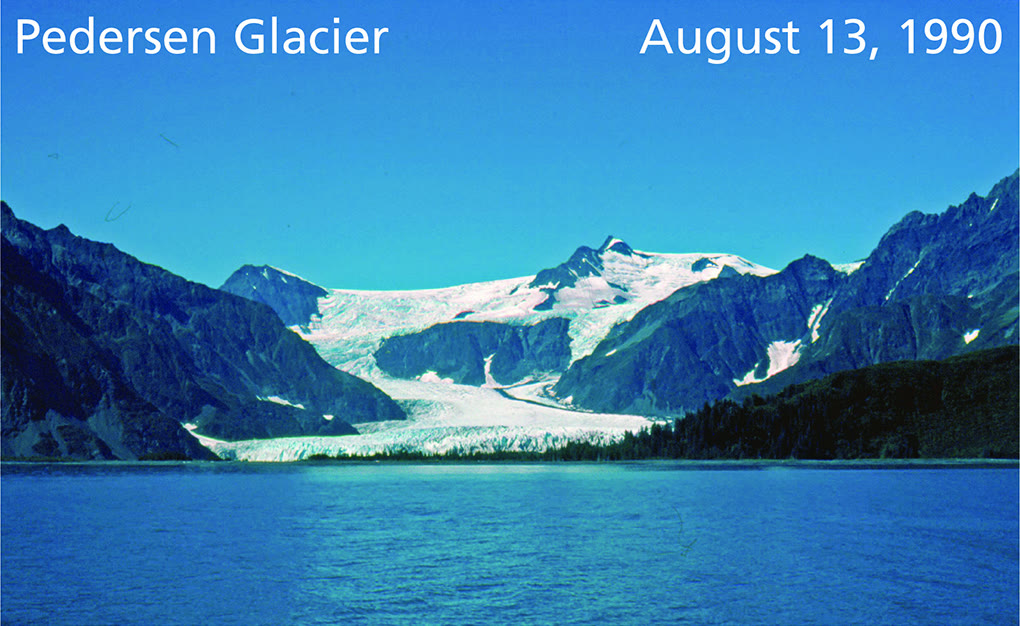
\includegraphics[width=\linewidth]{images/book1/g8-pedersen-1990.jpg}
\end{minipage}\hfill
\begin{minipage}[t]{0.49\linewidth}\centering
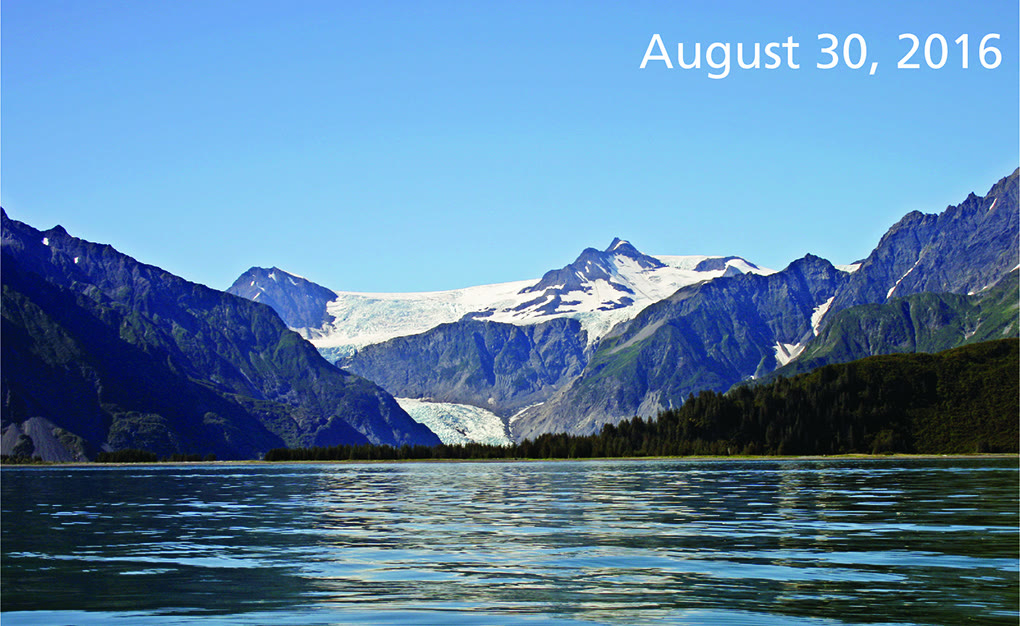
\includegraphics[width=\linewidth]{images/book1/g8-pedersen-2016.jpg}
\end{minipage}

\smallskip
{\small पेडरसन \omterm{def:g8:ice-on-earth:glacier}{हिमनद}, केनाई फ़्योर्ड्स राष्ट्रीय उद्यान, अलास्का, एक ही जगह से 13~अगस्त
1990 को (बाएँ, फ़ोटो: टेट्रो) और 30~अगस्त 2016 को (दाएँ, फ़ोटो: कुर्ट्ज़) देखा गया।
अमेरिकी राष्ट्रीय उद्यान सेवा, सार्वजनिक डोमेन (विकिमीडिया कॉमन्स के
ज़रिए)।}
% ledger: commons:pedersen
\label{fig:g8:ice-on-earth:pedersen}
\end{omfigure}

आज बर्फ़ पृथ्वी की ज़मीन के लगभग दसवें हिस्से को ढकती है। वह \omterm{def:g1:landscapes-around-us:landform}{पहाड़ी} \omterm{def:g1:landscapes-around-us:landform}{घाटियों} में, अंटार्कटिका
और ग्रीनलैंड के ऊपर दो विशाल चादरों में, ध्रुवीय \omterm{def:g2:water-on-earth:ocean}{समुद्रों} पर और, छिपी हुई, सुदूर उत्तर
की जमी हुई ज़मीन के अंदर है। यह अध्याय बारी-बारी से इनमें से हर एक को देखता है, यह
देखता है कि बर्फ़ ज़मीन को कैसे आकार देती है, और उन समयों को भी जब बर्फ़ ने पृथ्वी के
आज से कहीं ज़्यादा हिस्से को ढक रखा था।
% ledger: nsidc:ice-cover

\begin{recall}
\omterm{def:g4:clouds-rain-snow:precipitation}{हिम} \omterm{def:g4:clouds-rain-snow:precipitation}{वर्षण} का एक प्रकार है: बर्फ़ के क्रिस्टल जो \omterm{def:g4:clouds-rain-snow:cloud}{बादल} में बढ़ते हैं और बिना पिघले गिरते
हैं (\cref{ch:g4:clouds-rain-snow})। बहता पानी ज़मीन का \omterm{def:g5:water-shapes-the-land:erosion}{अपरदन} करता है, टुकड़ों को बहा
ले जाता है और उन्हें आगे नीचे जमा कर देता है; \omterm{def:g1:landscapes-around-us:water}{नदी} \omterm{def:g1:landscapes-around-us:landform}{घाटी} काटती है
(\cref{ch:g5:water-shapes-the-land})। जब समुद्री पानी जमता है, तो लवण बर्फ़ के
आसपास के पानी में पीछे छूट जाता है (\cref{ch:g8:the-oceans})। भौतिकी में तुम सीखते
हो कि जमने पर पानी फैलता है, इसलिए बर्फ़ तरल पानी से कम घनी होती है, और कि जो पिंड अपने
हटाए पानी से हल्का हो, वह तैरता
है।
\end{recall}

\section{हिमनद}

पहाड़ों में ऊँचे पर जाड़े में जितना \omterm{def:g4:clouds-rain-snow:precipitation}{हिम} गिरता है, उतना गर्मी में पिघलता नहीं। साल-दर-साल
नया \omterm{def:g4:clouds-rain-snow:precipitation}{हिम} पुराने \omterm{def:g4:clouds-rain-snow:precipitation}{हिम} को दबा देता है और उसे नीचे दबाता है। क्रिस्टल आपस में सटते जाते हैं,
उनके बीच की हवा निकल जाती है, और लगभग एक वर्ष बाद \omterm{def:g4:clouds-rain-snow:precipitation}{हिम} \emph{फ़िर्न} बन जाता है, जो
\omterm{def:g4:clouds-rain-snow:precipitation}{हिम} और बर्फ़ के बीच का एक दानेदार पदार्थ है। और गहरा दबते-दबते फ़िर्न कठोर, ठोस बर्फ़ में
बदल जाता है; ज़्यादातर \omterm{def:g8:ice-on-earth:glacier}{हिमनदों} में इसमें सौ से ज़्यादा वर्ष लगते
हैं।
% ledger: nsidc:firn

\begin{definition}[हिमनद]\label{def:g8:ice-on-earth:glacier}
\emph{हिमनद}\index{हिमनद} कई वर्षों में जमा हुए \omterm{def:g4:clouds-rain-snow:precipitation}{हिम} से बनी बर्फ़ की एक राशि है, जो
अपने ही भार से ज़मीन पर धीरे-धीरे ढलान से नीचे की ओर चलती है।
\end{definition}
% ledger: nsidc:glacier-def

\omterm{def:g8:ice-on-earth:glacier}{हिमनद} के दो हिस्से होते हैं। उसके ऊपरी हिस्से, \emph{संचयन क्षेत्र}, में हर वर्ष जितना
\omterm{def:g4:clouds-rain-snow:precipitation}{हिम} गिरता है, उससे कम पिघलता है: \omterm{def:g8:ice-on-earth:glacier}{हिमनद} बर्फ़ पाता है। उसके निचले हिस्से,
\emph{अपक्षरण क्षेत्र}, में हर वर्ष जितना \omterm{def:g4:clouds-rain-snow:precipitation}{हिम} गिरता है, उससे ज़्यादा बर्फ़ पिघलती है:
\omterm{def:g8:ice-on-earth:glacier}{हिमनद} बर्फ़ खोता है। ऊपर पाई गई बर्फ़ नीचे खोई बर्फ़ की जगह लेने के लिए लगातार नीचे बहती
रहती है। अगर दोनों बराबर हों, तो \omterm{def:g8:ice-on-earth:glacier}{हिमनद} का अगला सिरा, उसका \emph{मुख}, एक ही जगह
रहता है।
% ledger: nsidc:glacier-zones

\begin{omfigure}
\begin{tikzpicture}[font=\footnotesize, >={Stealth[length=2mm]}, xscale=1.08]
  % bedrock
  \fill[black!13] (0,4.6) -- (2,3.9) -- (4,3.0) -- (6,2.0) -- (8,1.1)
    -- (10,0.45) -- (11,0.3) -- (13,0.15) -- (13,-0.5) -- (0,-0.5) -- cycle;
  % the ice body, two zones
  \begin{scope}
    \clip (0,5.5) -- (2,4.9) -- (4,4.0) -- (6,2.9) -- (8,1.8) -- (9.4,0.95)
      -- (10,0.45) -- (8,1.1) -- (6,2.0) -- (4,3.0) -- (2,3.9) -- (0,4.6) -- cycle;
    \fill[omIce] (0,-1) rectangle (5,6);
    \fill[omSea!85] (5,-1) rectangle (11,6);
  \end{scope}
  \draw[black!60] (0,5.5) -- (2,4.9) -- (4,4.0) -- (6,2.9) -- (8,1.8)
    -- (9.4,0.95) -- (10,0.45);
  \draw[black!70, line width=0.6pt] (0,4.6) -- (2,3.9) -- (4,3.0) -- (6,2.0)
    -- (8,1.1) -- (10,0.45) -- (11,0.3) -- (13,0.15);
  % snowline
  \draw[dashed, black!70] (5,2.5) -- (5,4.15);
  \node[anchor=south] at (5,4.15) {हिमपात = पिघलना};
  % snowflakes and melting
  \foreach \x/\y in {0.5/6.1, 1.3/5.8, 2.1/5.5, 2.9/5.1, 3.7/4.8, 0.9/6.6, 1.7/6.3, 2.5/6.0, 3.3/5.6, 4.1/5.2}
    \node[omCold] at (\x,\y) {$\ast$};
  \foreach \x/\y in {6.4/2.8, 7.2/2.35, 8.0/1.9}
    \draw[omWarm, decorate, decoration={snake, amplitude=0.6mm, segment length=2mm}] (\x,\y) -- ++(0,0.6);
  % flow arrows inside the ice
  \draw[->, omDef, line width=0.9pt] (1.0,4.72) -- (2.2,4.30);
  \draw[->, omDef, line width=0.9pt] (3.0,3.95) -- (4.2,3.41);
  \draw[->, omDef, line width=0.9pt] (5.2,2.88) -- (6.4,2.28);
  \draw[->, omDef, line width=0.9pt] (7.2,1.84) -- (8.3,1.35);
  % moraine and meltwater
  \fill[omLithCongl] (10.15,0.42) .. controls (10.5,0.95) and (10.9,0.95) .. (11.2,0.29) -- cycle;
  \draw[omSea!60!black, line width=1.6pt] (10.05,0.38) .. controls (10.6,0.22) and (11.4,0.12) .. (12.9,0.08);
  % labels
  \node[align=center] at (1.9,7.15) {संचयन क्षेत्र:\\ हिम जमा होता है, हिमनद बर्फ़ पाता है};
  \node[align=center] at (10.0,3.3) {अपक्षरण क्षेत्र:\\ बर्फ़ पिघलती है, हिमनद बर्फ़ खोता है};
  \node[align=left, anchor=west, omDef] at (4.4,1.3) {बर्फ़ ढलान से\\ नीचे बहती है};
  \draw[black!60] (10.0,0.5) -- (9.6,-0.1) node[below] {मुख};
  \draw[black!60] (10.7,0.85) -- (11.3,1.4) node[above] {हिमोढ़};
  \node[anchor=north east] at (12.9,0.0) {पिघले पानी की धारा};
  \node at (2.2,2.6) {आधार शैल};
\end{tikzpicture}

{\small लंबी काट में देखा गया एक \omterm{def:g1:landscapes-around-us:landform}{घाटी} \omterm{def:g8:ice-on-earth:glacier}{हिमनद} (एक रेखाचित्र, पैमाने पर नहीं)। टूटी रेखा के
ऊपर \omterm{def:g4:clouds-rain-snow:precipitation}{हिम} पिघलने से ज़्यादा तेज़ी से जमा होता है; उसके नीचे बर्फ़ \omterm{def:g4:clouds-rain-snow:precipitation}{हिम} गिरने से ज़्यादा तेज़ी से
पिघलती है। बर्फ़ एक हिस्से से दूसरे हिस्से की ओर नीचे
बहती है।}
\label{fig:g8:ice-on-earth:long-section}
\end{omfigure}

ठोस बर्फ़ कैसे बह सकती है? अपने ऊपर की बर्फ़ के भार से \omterm{def:g8:ice-on-earth:glacier}{हिमनद} के गहरे हिस्से की बर्फ़
धीरे-धीरे आकार बदलती है, उसी तरह जैसे ठंडे शहद की एक मोटी परत फैलती है। \omterm{def:g8:ice-on-earth:glacier}{हिमनद} अपने नीचे
की \omterm{def:g3:stones-pebbles-sand:rock}{चट्टान} पर भी, पानी की एक पतली परत या गीली \omterm{def:g3:stones-pebbles-sand:sand}{कीचड़} पर, फिसलता है। \omterm{def:g3:stones-pebbles-sand:rock}{चट्टान} से रगड़ खाता
\omterm{def:g8:ice-on-earth:glacier}{हिमनद} का तला उसके ऊपरी हिस्से से धीमा चलता है। ज़्यादातर \omterm{def:g8:ice-on-earth:glacier}{हिमनद} धीरे और लगातार चलते हैं;
कुछ अचानक \emph{उमड़ पड़ते} हैं। 1986 में अलास्का का हबर्ड \omterm{def:g8:ice-on-earth:glacier}{हिमनद} लगभग \qty{10}{m}
प्रति दिन आगे उमड़ा, और दर्ज सबसे तेज़ उमड़, 1953 में पाकिस्तान के कुटियाह \omterm{def:g8:ice-on-earth:glacier}{हिमनद} की, तीन
महीनों तक औसतन लगभग \qty{112}{m} प्रति दिन
रही।
% ledger: nsidc:glacier-flow, nsidc:surges

जब कोई \omterm{def:g8:ice-on-earth:glacier}{हिमनद} ऊपर जितनी बर्फ़ पाता है, उससे ज़्यादा नीचे खोता है, तो उसका मुख \omterm{def:g1:landscapes-around-us:landform}{घाटी} में ऊपर
की ओर पीछे खिसकता है: \omterm{def:g8:ice-on-earth:glacier}{हिमनद} \emph{पीछे हटता} है। पीछे हटता \omterm{def:g8:ice-on-earth:glacier}{हिमनद} भी एक कन्वेयर बेल्ट
की तरह ढलान से नीचे बहता रहता है; बस वह जितना बहता है, उससे तेज़ पिघलता है। अलास्का का
म्यूर \omterm{def:g8:ice-on-earth:glacier}{हिमनद} 1941 में अपनी पूरी \omterm{def:g1:landscapes-around-us:landform}{घाटी} को \omterm{def:g2:water-on-earth:ocean}{समुद्र} तक भरे हुए था। 2004 तक उसका मुख
\qty{12}{km} पीछे हट गया था, और बर्फ़ की सतह \qty{800}{m} से ज़्यादा नीचे आ गई
थी।
% ledger: nsidc:glacier-flow, nsidc:muir

\section{बर्फ़ घाटी को कैसे आकार देती है}

\omterm{def:g8:ice-on-earth:glacier}{हिमनद} \omterm{def:g5:water-shapes-the-land:erosion}{अपरदन} का एक शक्तिशाली औज़ार है। उसकी बर्फ़ ढीली \omterm{def:g3:stones-pebbles-sand:rock}{चट्टान} के खंडों पर जम जाती है और
उन्हें उखाड़ लेती है; उसके तले में जमे पत्थर नीचे की \omterm{def:g3:stones-pebbles-sand:rock}{चट्टान} को रेगमाल की तरह खुरचते हैं।
\omterm{def:g8:ice-on-earth:glacier}{हिमनद} यह सारी \omterm{def:g3:stones-pebbles-sand:rock}{चट्टान}, महीन धूल से लेकर विशाल शिलाखंडों तक, एक कन्वेयर बेल्ट की तरह \omterm{def:g1:landscapes-around-us:landform}{घाटी}
में नीचे ले जाता है, और जहाँ बर्फ़ पिघलती है वहाँ गिरा देता
है।
% ledger: nps:u-valley

\begin{omfigure}
\begin{tikzpicture}[font=\footnotesize, >={Stealth[length=2mm]}]
  % V-shaped valley
  \fill[black!13] (0,3) -- (2.1,0.35) -- (2.5,0.35) -- (4.6,3) -- (4.6,-0.4) -- (0,-0.4) -- cycle;
  \draw[black!70, line width=0.6pt] (0,3) -- (2.1,0.35) -- (2.5,0.35) -- (4.6,3);
  \fill[omSea] (2.1,0.35) -- (2.5,0.35) -- (2.42,0.2) -- (2.18,0.2) -- cycle;
  \node[align=center] at (2.3,-0.85) {नदी एक संकरी\\ V-आकार की घाटी काटती है};
  % arrow
  \draw[->, line width=1pt] (5.0,1.5) -- (6.2,1.5) node[midway, above, align=center] {हिमनद\\ उसे भरता है};
  % U-shaped valley
  \begin{scope}[xshift=6.6cm]
    \fill[black!13] (0,3) .. controls (0.6,1.0) and (0.9,0.25) .. (1.6,0.2)
      -- (3.0,0.2) .. controls (3.7,0.25) and (4.0,1.0) .. (4.6,3) -- (4.6,-0.4) -- (0,-0.4) -- cycle;
    \draw[black!70, line width=0.6pt] (0,3) .. controls (0.6,1.0) and (0.9,0.25) .. (1.6,0.2)
      -- (3.0,0.2) .. controls (3.7,0.25) and (4.0,1.0) .. (4.6,3);
    \draw[dashed, black!40] (0,3) -- (2.1,0.35) -- (2.5,0.35) -- (4.6,3);
    \draw[omCold, line width=0.9pt] (0.37,2.2) -- (4.23,2.2);
    \node[omCold, anchor=south, font=\scriptsize] at (2.3,2.2) {बहुत पहले बर्फ़ की सतह};
    \fill[omLithCongl] (0.75,0.95) .. controls (0.95,1.2) and (1.1,1.1) .. (1.2,0.6) -- cycle;
    \fill[omLithCongl] (3.85,0.95) .. controls (3.65,1.2) and (3.5,1.1) .. (3.4,0.6) -- cycle;
    \node[align=center] at (2.3,-0.85) {बर्फ़ जाने के बाद: एक चौड़ी\\ U-आकार की घाटी, खड़ी ढलानें};
    \draw[black!60] (3.65,0.95) -- (4.85,0.6) node[right, align=left] {पार्श्व\\ हिमोढ़};
    \node[font=\scriptsize, black!55, align=center] at (2.3,1.6) {(पुराना V टूटी रेखा में)};
  \end{scope}
\end{tikzpicture}

{\small वही \omterm{def:g1:landscapes-around-us:landform}{पहाड़ी} \omterm{def:g1:landscapes-around-us:landform}{घाटी} अनुप्रस्थ काट में, \omterm{def:g8:ice-on-earth:glacier}{हिमनद} से पहले और बाद में (एक रेखाचित्र)। बर्फ़
संकरी नदी-घाटी को खुरचकर चौड़े तल और खड़ी ढलानों वाली एक चौड़ी द्रोणी बना देती है, और
अपने किनारों के साथ-साथ चट्टानी मलबे की मेड़ें छोड़
जाती है।}
\label{fig:g8:ice-on-earth:v-and-u}
\end{omfigure}

\begin{definition}[U-आकार की घाटी और हिमोढ़]\label{def:g8:ice-on-earth:glacial-landforms}
\emph{U-आकार की घाटी}\index{U-आकार की घाटी} चौड़े, समतल तल और खड़ी ढलानों वाली \omterm{def:g1:landscapes-around-us:landform}{घाटी}
है, जिसे किसी \omterm{def:g8:ice-on-earth:glacier}{हिमनद} ने एक संकरी V-आकार की नदी-घाटी को चौड़ा और गहरा करके तराशा है।
\emph{हिमोढ़}\index{हिमोढ़} \omterm{def:g8:ice-on-earth:glacier}{हिमनद} का छोड़ा हुआ, धूल से लेकर शिलाखंडों तक के चट्टानी
मलबे का एक मेड़ है: उसके किनारे के साथ \emph{पार्श्व हिमोढ़}, उसके छोर पर
\emph{अंतस्थ हिमोढ़}।
\end{definition}
% ledger: usgs:erratic, nps:u-valley, nps:moraines

\omterm{def:g8:ice-on-earth:glacial-landforms}{हिमोढ़} काम के सुराग हैं। \omterm{def:g1:landscapes-around-us:landform}{घाटी} में बहुत नीचे एक अंतस्थ \omterm{def:g8:ice-on-earth:glacial-landforms}{हिमोढ़}, जिसके आसपास कहीं बर्फ़ न हो,
दिखाता है कि \omterm{def:g8:ice-on-earth:glacier}{हिमनद} कभी कहाँ तक पहुँचता था; \omterm{def:g1:landscapes-around-us:landform}{घाटी} की ढलान पर ऊँचे पर एक पार्श्व \omterm{def:g8:ice-on-earth:glacial-landforms}{हिमोढ़}
दिखाता है कि बर्फ़ कभी कितनी मोटी थी। किसी खेत में अकेला पड़ा एक बड़ा शिलाखंड, जो ऐसी
\omterm{def:g3:stones-pebbles-sand:rock}{चट्टान} का बना हो जो आसपास कहीं न मिलती हो, एक और सुराग है: वह एक \emph{अनियत शिला}
है, एक ऐसी \omterm{def:g3:stones-pebbles-sand:rock}{चट्टान} जिसे \omterm{def:g8:ice-on-earth:glacier}{हिमनद} उसके घर से दूर ले गया और बर्फ़ पिघलने पर पीछे छोड़ गया।
अनियत शिलाएँ \omterm{def:g3:stones-pebbles-sand:pebble}{कंकड़ों} से लेकर घर से बड़े खंडों तक होती
हैं।
% ledger: nps:moraines, usgs:erratic

\begin{inthefield}[बर्फ़ से आकार पाई घाटी पढ़ना]
पहाड़ों में सैर के दौरान, या किसी \omterm{def:g1:landscapes-around-us:landform}{पहाड़ी} \omterm{def:g1:landscapes-around-us:landform}{घाटी} की तस्वीर में, अनुप्रस्थ काट में \omterm{def:g1:landscapes-around-us:landform}{घाटी} का
आकार देखो: एक संकरा V, या खड़ी दीवारों वाला एक चौड़ा U? \omterm{def:g1:landscapes-around-us:landform}{घाटी} के तल पर उलझे-पुलझे
पत्थरों और मिट्टी की लंबी मेड़ें ढूँढो जो उसके किनारों के साथ या उसके आर-पार चलती हों:
वे \omterm{def:g8:ice-on-earth:glacial-landforms}{हिमोढ़} हो सकती हैं। ऐसे बड़े शिलाखंड ढूँढो जो आसपास की \omterm{def:g3:stones-pebbles-sand:rock}{चट्टान} से मेल न खाते हों, और
लंबी समानांतर रेखाओं से खरोंची चिकनी चट्टानी सतहें। पगडंडियों पर रहो, खड़ी ढलानों के
किनारों से और ख़ुद बर्फ़ से दूर रहो, और जो दिखे उसे अपनी नोटबुक में
बनाओ।
\end{inthefield}

\section{हिमचादरें, हिम शेल्फ़ और हिमशैल}

पृथ्वी पर बर्फ़ की सबसे बड़ी राशियाँ \omterm{def:g1:landscapes-around-us:landform}{पहाड़ी} \omterm{def:g1:landscapes-around-us:landform}{घाटियों} में नहीं हैं: वे पूरे-के-पूरे भूभाग
ढकती हैं। अंटार्कटिका की \omterm{def:g8:ice-on-earth:ice-sheet}{हिमचादर} लगभग \num{14}~मिलियन~\unit{km^2} पर फैली है और अपने
सबसे मोटे हिस्से में लगभग \qty{4.9}{km} मोटी है। ग्रीनलैंड की \omterm{def:g8:ice-on-earth:ice-sheet}{हिमचादर} लगभग
\num{1.7}~मिलियन~\unit{km^2} ढकती है, द्वीप का चार-पाँचवाँ हिस्सा, और \qty{3}{km} से
ज़्यादा मोटी है। दोनों मिलकर ज़मीन की 99~\% से ज़्यादा बर्फ़, और पृथ्वी के सारे \omterm{def:g2:water-on-earth:salt-fresh}{मीठे पानी}
का दो-तिहाई से ज़्यादा हिस्सा, रखती
हैं।
% ledger: nsidc:ice-sheets

\begin{definition}[हिमचादर, हिम शेल्फ़ और हिमशैल]\label{def:g8:ice-on-earth:ice-sheet}
\emph{हिमचादर}\index{हिमचादर} \qty{50000}{km^2} से ज़्यादा ज़मीन को ढकने वाली बर्फ़ की
एक राशि है, एक विशाल गुंबद की तरह जो सब दिशाओं में बाहर की ओर फैलता है। जहाँ ज़मीन से
बहती बर्फ़ \omterm{def:g2:water-on-earth:ocean}{समुद्र} तक पहुँचती है और उस पर तैरती चली जाती है, पीछे की बर्फ़ से जुड़ी
रहकर, वहाँ वह एक \emph{हिम शेल्फ़}\index{हिम शेल्फ़} बनाती है। \emph{हिमशैल}\index{हिमशैल}
बर्फ़ का एक बड़ा खंड है, \qty{5}{m} से ज़्यादा चौड़ा, जो किसी \omterm{def:g8:ice-on-earth:glacier}{हिमनद} या \omterm{def:g4:clouds-rain-snow:precipitation}{हिम} शेल्फ़ से
टूटकर अलग हुआ है और \omterm{def:g2:water-on-earth:ocean}{समुद्र} में तैरता
है।
\end{definition}
% ledger: nsidc:ice-sheets, nsidc:ice-shelves, nsidc:iceberg

\begin{omfigure}
\begin{minipage}[c]{0.5\linewidth}\centering
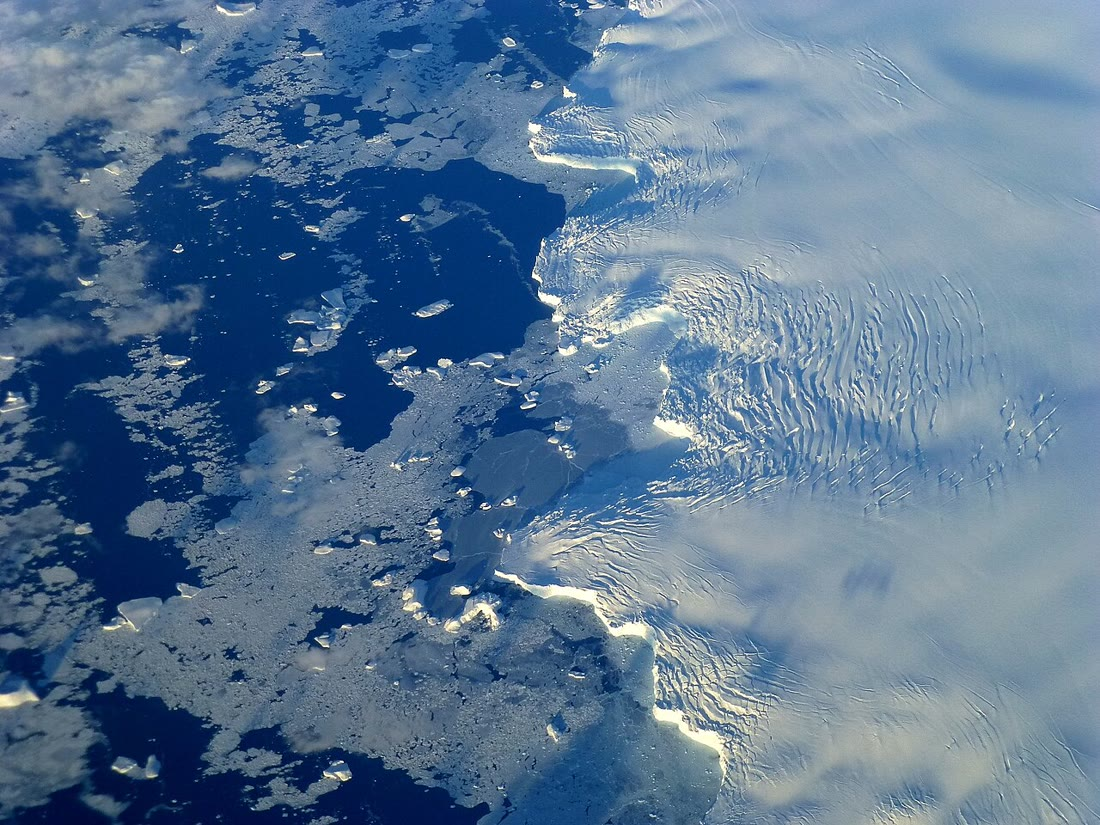
\includegraphics[width=\linewidth]{images/book1/g8-ice-shelf-edge.jpg}
\end{minipage}\hfill
\begin{minipage}[c]{0.46\linewidth}\raggedright
{\small अंटार्कटिक प्रायद्वीप के सामने, एडिलेड द्वीप के पास एक \omterm{def:g8:ice-on-earth:ice-sheet}{हिम शेल्फ़} का किनारा, जिसे
28~अक्टूबर 2012 को एक विमान से देखा गया। दाईं ओर की मोटी, सिलवटों वाली सफ़ेद बर्फ़ \omterm{def:g8:ice-on-earth:ice-sheet}{हिम
शेल्फ़} है; बाईं ओर पतली \omterm{def:g8:ice-on-earth:sea-ice}{समुद्री बर्फ़} के टूटे टुकड़े गहरे पानी पर तैर रहे हैं। NASA,
ऑपरेशन आइसब्रिज (सार्वजनिक डोमेन, विकिमीडिया कॉमन्स के
ज़रिए)।}
\end{minipage}
% ledger: commons:ice-shelf
\label{fig:g8:ice-on-earth:ice-shelf}
\end{omfigure}

\omterm{def:g8:ice-on-earth:ice-sheet}{हिमचादरों} में बंद पानी \omterm{def:g2:water-on-earth:ocean}{महासागर} से आया था: वह भाप बनकर उड़ा, \omterm{def:g4:clouds-rain-snow:precipitation}{हिम} बनकर गिरा और ज़मीन पर
जमा होता गया। अगर ग्रीनलैंड की सारी बर्फ़ पिघल जाए, तो \omterm{def:g2:water-on-earth:ocean}{समुद्र} लगभग \qty{7.4}{m} ऊपर उठ
जाएगा; अगर अंटार्कटिका की सारी बर्फ़ पिघल जाए, तो लगभग \qty{58}{m}। दुनिया के सारे
\omterm{def:g1:landscapes-around-us:landform}{पहाड़ी} \omterm{def:g8:ice-on-earth:glacier}{हिमनद}, जो \num{200000} से ज़्यादा हैं, आधे मीटर से भी कम
जोड़ेंगे।
% ledger: nsidc:ice-sheets, nsidc:ice-cover

\begin{omfigure}
\begin{tikzpicture}
\begin{axis}[omrecord, xbar, width=10.5cm, height=3.6cm, xmin=0, xmax=68,
  bar width=9pt, ytick=data, symbolic y coords={glaciers,Greenland,Antarctica},
  yticklabels={सारे पहाड़ी हिमनद, ग्रीनलैंड की हिमचादर, अंटार्कटिका की हिमचादर},
  xlabel={सब कुछ पिघल जाए तो समुद्र का उठना (m)}, enlarge y limits=0.3,
  nodes near coords, nodes near coords style={font=\footnotesize, anchor=west, fill=white, inner sep=1.5pt},
  ymajorgrids=false]
  \addplot[fill=omIce!80!black, draw=black!60] coordinates {(0.5,glaciers) (7.4,Greenland) (58,Antarctica)};
\end{axis}
\end{tikzpicture}

{\small अगर ज़मीन की बर्फ़ का हर प्रकार पूरी तरह पिघल जाए तो \omterm{def:g2:water-on-earth:ocean}{समुद्र} कितना ऊपर उठेगा
(मान अमेरिका के राष्ट्रीय \omterm{def:g4:clouds-rain-snow:precipitation}{हिम} और बर्फ़ आँकड़ा केंद्र से; \omterm{def:g8:ice-on-earth:glacier}{हिमनदों} का मान एक ऊपरी सीमा
है, ``आधे मीटर से थोड़ा कम'')।}
% ledger: nsidc:ice-sheets, nsidc:ice-cover
\label{fig:g8:ice-on-earth:sea-level-bars}
\end{omfigure}

तैरती बर्फ़ अलग है। \omterm{def:g8:ice-on-earth:ice-sheet}{हिम शेल्फ़} या \omterm{def:g8:ice-on-earth:ice-sheet}{हिमशैल} पहले से \omterm{def:g2:water-on-earth:ocean}{समुद्र} पर तैर रहा है: वह अपने भार जितना
पानी पहले ही हटा चुका है। जब वह टूटता या पिघलता है, तो \omterm{def:g2:water-on-earth:ocean}{समुद्र} ऊपर नहीं उठता। पर \omterm{def:g8:ice-on-earth:ice-sheet}{हिम
शेल्फ़} अपने पीछे के \omterm{def:g8:ice-on-earth:glacier}{हिमनदों} को रोके रखती है, बोतल में डाट की तरह; जब 2002 में
अंटार्कटिका की लार्सन~B \omterm{def:g8:ice-on-earth:ice-sheet}{हिम शेल्फ़} टूटकर बिखर गई, तो उसके पीछे के \omterm{def:g8:ice-on-earth:glacier}{हिमनद} तेज़ हो गए,
कुछ अपनी पहले की चाल से आठ गुना तक, और उन्होंने ज़मीन की और ज़्यादा बर्फ़ \omterm{def:g2:water-on-earth:ocean}{समुद्र} में
उड़ेल दी।
% ledger: nsidc:ice-shelves

\begin{inthelab}[तैरती बर्फ़ और ज़मीन पर की बर्फ़]
घर के अंदर, दो पारदर्शी गिलासों में से हर एक में एक छोटा पत्थर ऐसे रखो कि गिलास भरने
पर वह पानी से ऊपर निकला रहे। पहले गिलास में पानी पर कुछ बर्फ़ के टुकड़े तैराओ। दूसरे
में उतने ही बर्फ़ के टुकड़े पत्थर पर, पानी से बाहर, टिकाओ। दोनों गिलासों में एक ही स्तर
तक पानी भरो और फ़ेल्ट पेन से उसका निशान लगाओ। सारी बर्फ़ पिघलने तक रुको, फिर पानी के
स्तरों की निशानों से तुलना करो। कौन-सा गिलास \omterm{def:g8:ice-on-earth:ice-sheet}{हिमशैल} पिघलने पर \omterm{def:g2:water-on-earth:ocean}{समुद्र} की तरह बरताव करता
है, और कौन-सा \omterm{def:g8:ice-on-earth:ice-sheet}{हिमचादर} पिघलने पर \omterm{def:g2:water-on-earth:ocean}{समुद्र} की
तरह?
\end{inthelab}

\section{समुद्री बर्फ़}

\omterm{def:g8:ice-on-earth:sea-ice}{समुद्री बर्फ़} फिर कुछ और है: वह ख़ुद जमा हुआ \omterm{def:g2:water-on-earth:ocean}{समुद्र} है। हर जाड़े में ध्रुवीय \omterm{def:g2:water-on-earth:ocean}{महासागरों} की
सतह एक विशाल क्षेत्र पर जम जाती है; हर गर्मी में इस बर्फ़ का बहुत-सा हिस्सा फिर पिघल
जाता है। आर्कटिक में बर्फ़ गर्मी के अंत में, सितंबर में, सबसे कम होती है, और जाड़े के
अंत में, मार्च में, सबसे ज़्यादा। उपग्रहों ने 1970 के दशक के आख़िरी वर्षों से हर दिन
उसका \emph{विस्तार} मापा है, यानी \omterm{def:g2:water-on-earth:ocean}{समुद्र} का वह क्षेत्र जहाँ सतह का कम से कम 15~\%
बर्फ़ से ढका हो।
% ledger: nsidc:sea-ice-def

\begin{definition}[समुद्री बर्फ़]\label{def:g8:ice-on-earth:sea-ice}
\emph{समुद्री बर्फ़}\index{समुद्री बर्फ़} जमा हुआ समुद्री पानी है: वह ख़ुद \omterm{def:g2:water-on-earth:ocean}{महासागर} में
बनती, बढ़ती और पिघलती है। वह \omterm{def:g8:ice-on-earth:ice-sheet}{हिमशैलों} और \omterm{def:g8:ice-on-earth:ice-sheet}{हिम शेल्फ़ों} से अलग है, जो \omterm{def:g2:water-on-earth:ocean}{समुद्र} पर तैरते
हैं पर ज़मीन पर गिरे \omterm{def:g4:clouds-rain-snow:precipitation}{हिम} से बने थे।
\end{definition}
% ledger: nsidc:sea-ice-def

\omterm{def:g8:ice-on-earth:sea-ice}{समुद्री बर्फ़} \omterm{def:g3:continents-and-oceans:poles}{ध्रुवों} से बहुत दूर तक मायने रखती है। खुला समुद्री पानी गहरे रंग का होता है:
वह उस तक पहुँचने वाले सूर्य के प्रकाश का केवल लगभग 6~\% परावर्तित करता है और बाकी
सोख लेता है। \omterm{def:g8:ice-on-earth:sea-ice}{समुद्री बर्फ़} 50 से 70~\% परावर्तित करती है, और \omterm{def:g4:clouds-rain-snow:precipitation}{हिम} से ढकी \omterm{def:g8:ice-on-earth:sea-ice}{समुद्री बर्फ़}
90~\% तक। जब बर्फ़ पिघलती है, तो नीचे का गहरा पानी सूर्य की ज़्यादा ऊर्जा सोखता है और
गरम होता है, जिससे और बर्फ़ पिघलती है।
% ledger: nsidc:sea-ice-reflect

\begin{omfigure}
\begin{tikzpicture}
\begin{axis}[omrecord, width=13cm, height=5.4cm, xmin=1977, xmax=2027,
  ymin=3, ymax=8.2, xtick={1980,1990,...,2020},
  x tick label style={/pgf/number format/1000 sep={}},
  xlabel={वर्ष}, ylabel={विस्तार (मिलियन km$^2$)},
  legend style={at={(0.98,0.97)}, anchor=north east, draw=none, fill=white}]
  \addplot[omCold, mark=*, mark size=1.3pt, line width=0.6pt]
    table[x=year, y=extent_Mkm2] {figdata/out/grade-8-sea_ice-extent.dat};
  \addlegendentry{सितंबर का औसत विस्तार}
  \addplot[omWarm, dashed, line width=1pt]
    table[x=year, y=extent_Mkm2] {figdata/out/grade-8-sea_ice-trend.dat};
  \addlegendentry{प्रवृत्ति रेखा}
  \node[font=\scriptsize, anchor=north] at (axis cs:2012,3.5) {2012};
\end{axis}
\end{tikzpicture}

{\small हर सितंबर में आर्कटिक \omterm{def:g8:ice-on-earth:sea-ice}{समुद्री बर्फ़} का विस्तार, 1979--2025, और वह सीधी रेखा जो
बिंदुओं के सबसे पास चलती है। आँकड़े: NSIDC \omterm{def:g8:ice-on-earth:sea-ice}{समुद्री बर्फ़} सूचकांक, संस्करण~4 (फ़ेटरर
और अन्य, 2025)।}
% ledger: data:b1-nsidc-sea-ice (figdata/grade-8/sea_ice.py)
\label{fig:g8:ice-on-earth:sea-ice}
\end{omfigure}

बिंदु एक वर्ष से अगले वर्ष तक ऊपर-नीचे होते हैं: हर गर्मी का मौसम मायने रखता है। पर वर्षों
के साथ वे साफ़ तौर पर नीचे आते हैं। उतार-चढ़ाव के बीच बदलाव को देखने के लिए वैज्ञानिक एक
\emph{प्रवृत्ति रेखा} खींचते हैं, वह सीधी रेखा जो सभी बिंदुओं के जितना हो सके उतने पास
से गुज़रती है।
% ledger: data:b1-nsidc-sea-ice (figdata/grade-8/sea_ice.py)

\begin{method}[ग्राफ़ पर प्रवृत्ति पढ़ना]
\begin{enumerate}
  \item अक्ष पढ़ो: क्या मापा गया है, किस इकाई में, किन वर्षों में।
  \item बिंदुओं को देखो: उतार-चढ़ाव के पीछे क्या एक सामान्य बढ़त है, एक सामान्य
        गिरावट है, या दोनों में से कुछ नहीं?
  \item पहले वर्ष पर और आख़िरी वर्ष पर प्रवृत्ति रेखा पढ़ो।
  \item अंतर निकालो, और उसे उनके बीच के वर्षों (या दशकों) की संख्या से भाग दो: यह प्रति
        वर्ष (या प्रति दशक) औसत बदलाव
        है।
  \item किसी एक वर्ष से बहुत ज़्यादा मत निकालो: रेखा से दूर का कोई अकेला बिंदु \omterm{def:g1:watching-the-weather:weather}{मौसम} है,
        रेखा प्रवृत्ति है।
\end{enumerate}
\end{method}

\begin{example}[आर्कटिक की सितंबर की बर्फ़]
ग्राफ़ पर प्रवृत्ति रेखा 1979 में लगभग \num{7.6}~मिलियन~\unit{km^2} पर और 2025 में
लगभग \num{4.1}~मिलियन~\unit{km^2} पर है। बदलाव $7.6 - 4.1 =
3.5$ मिलियन~km$^2$
है, $2025 - 1979 = 46$ वर्षों में, यानी 4.6 दशकों में: $3.5 \div 4.6 \approx 0.76$।
सितंबर की \omterm{def:g8:ice-on-earth:sea-ice}{समुद्री बर्फ़} लगभग \num{0.76}~मिलियन~\unit{km^2} प्रति दशक सिकुड़ी है: 46
वर्षों में प्रवृत्ति रेखा ने अपने 1979 के मान का लगभग आधा खो दिया है। सबसे नीचा बिंदु,
2012 में \num{3.57}~मिलियन~\unit{km^2}, रेखा से काफ़ी नीचे है: वह गर्मी असाधारण
थी।
\end{example}
% ledger: data:b1-nsidc-sea-ice (figdata/grade-8/sea_ice.py), nsidc:sea-ice-reflect

माप दिखाते हैं कि 1980 के दशक से आर्कटिक की गर्मियों की \omterm{def:g8:ice-on-earth:sea-ice}{समुद्री बर्फ़} छोटी भी हुई है और
पतली भी, जबकि आर्कटिक गरम हुआ है। \Cref{ch:g9:climate-past-and-present} देखता है कि
पृथ्वी की \omterm{def:g5:weather-and-climate:climate}{जलवायु} कैसे बदल रही है, और
क्यों।
% ledger: nsidc:sea-ice-reflect

\section{पर्माफ़्रॉस्ट}

सुदूर उत्तर में ठंड ज़मीन में गहरे तक पहुँचती है। उत्तर अमेरिका, ग्रीनलैंड और उत्तरी
एशिया के टुंड्रा के नीचे मिट्टी और \omterm{def:g3:stones-pebbles-sand:rock}{चट्टान} पूरे वर्ष जमी रहती हैं, और अक्सर हज़ारों वर्षों
से जमी हुई हैं। केवल एक पतली ऊपरी परत, \emph{सक्रिय परत}, हर गर्मी में पिघलती है और
हर जाड़े में फिर जम जाती है; उसमें पौधे उगते हैं, और जो पानी नीचे की जमी ज़मीन में रिस
नहीं पाता, वह सतह पर पोखरों में भरा रहता
है।
% ledger: nsidc:permafrost

\begin{definition}[पर्माफ़्रॉस्ट]\label{def:g8:ice-on-earth:permafrost}
\emph{पर्माफ़्रॉस्ट}\index{पर्माफ़्रॉस्ट} वह ज़मीन, मिट्टी या \omterm{def:g3:stones-pebbles-sand:rock}{चट्टान}, है जो लगातार कम से
कम दो वर्ष \qty{0}{\degreeCelsius} पर या उससे नीचे रहती है।
\end{definition}
% ledger: nsidc:permafrost

\omterm{def:g8:ice-on-earth:permafrost}{पर्माफ़्रॉस्ट} लगभग \num{23}~मिलियन~\unit{km^2} के नीचे है, जो \omterm{def:g3:continents-and-oceans:equator}{उत्तरी गोलार्ध} की ज़मीन का
एक चौथाई है, और अलास्का के लगभग 85~\% के नीचे। बर्फ़ से भरी जमी ज़मीन \omterm{def:g3:stones-pebbles-sand:rock}{चट्टान} जितनी
कठोर होती है; जब उसकी बर्फ़ पिघलती है, तो ज़मीन \omterm{def:g3:stones-pebbles-sand:sand}{कीचड़} बनकर धँस जाती है। सड़कों में दरारें
पड़ती हैं, इमारतें झुक जाती हैं, और पाइपलाइनें टूट सकती हैं: जहाँ ट्रांस-अलास्का
पाइपलाइन \omterm{def:g8:ice-on-earth:permafrost}{पर्माफ़्रॉस्ट} को पार करती है, वहाँ वह \qty{676}{km} तक ज़मीन के ऊपर चलती है।
पिघलता \omterm{def:g8:ice-on-earth:permafrost}{पर्माफ़्रॉस्ट} उसमें हज़ारों वर्षों से जमे पौधों के अवशेषों को सड़ने भी देता है, और
वे हवा में कार्बन डाइऑक्साइड और मीथेन छोड़ते
हैं।
% ledger: nsidc:permafrost, nsidc:permafrost-thaw

\begin{omfigure}
\begin{minipage}[c]{0.5\linewidth}\centering
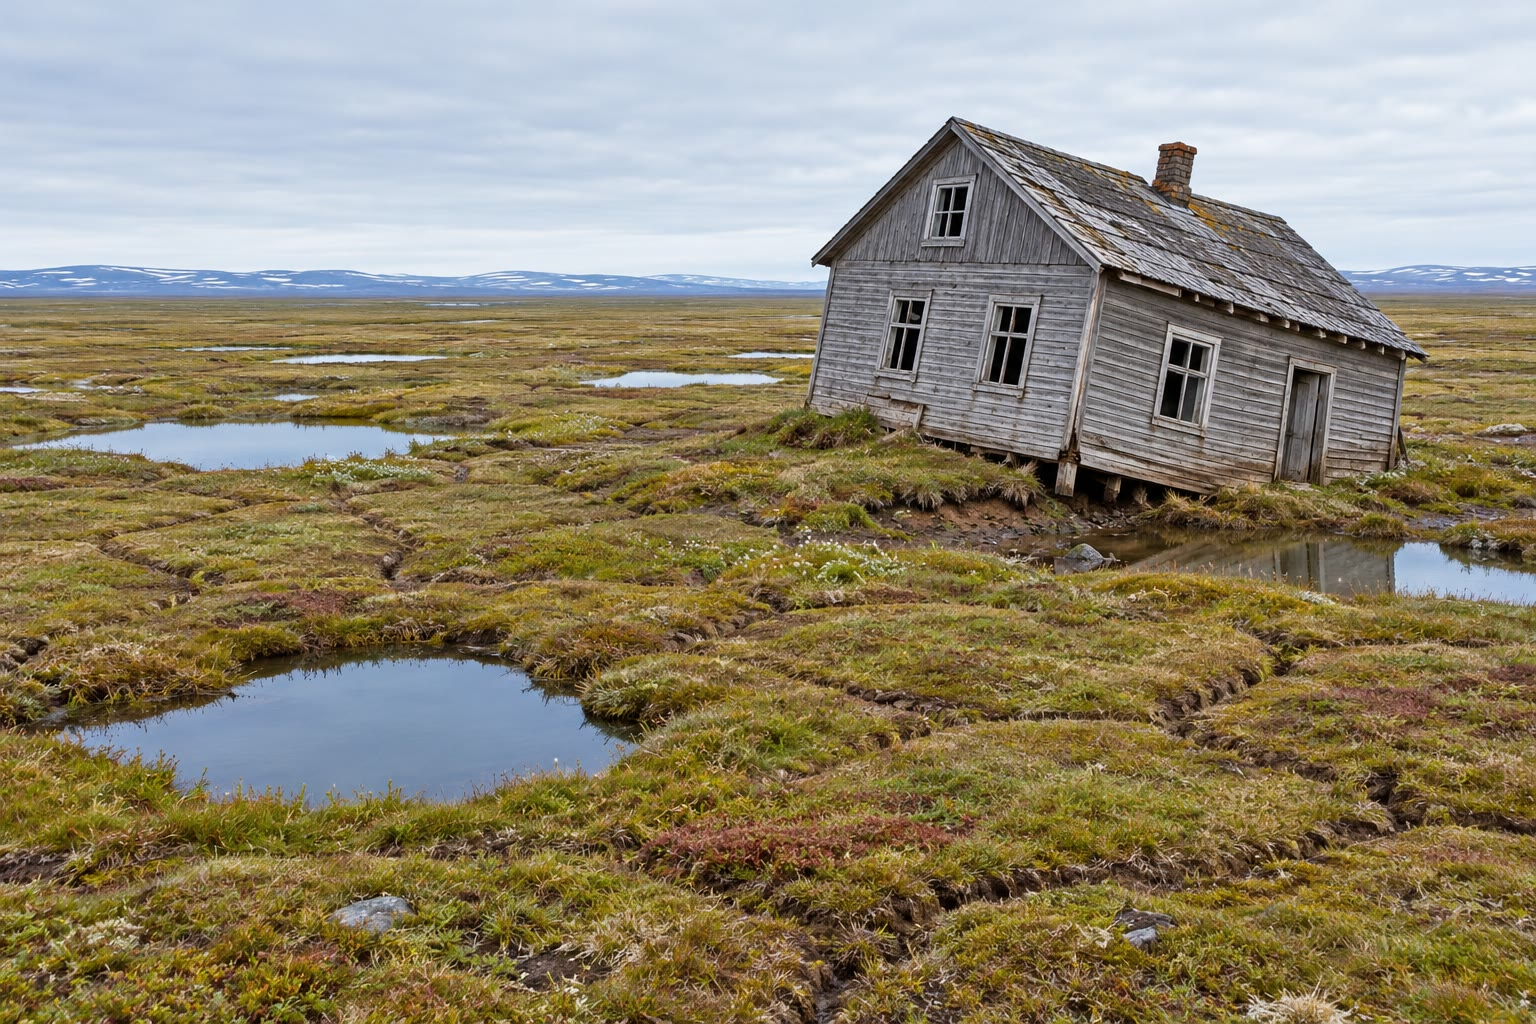
\includegraphics[width=\linewidth]{images/book1/ai/g8-permafrost-house.jpg}
\end{minipage}\hfill
\begin{minipage}[c]{0.46\linewidth}\centering
\begin{tikzpicture}[font=\footnotesize]
  \fill[omLithAlluv] (0,0) rectangle (3.2,-0.6);
  \fill[omIce!70!omLithShale] (0,-0.6) rectangle (3.2,-3.0);
  \foreach \x/\y in {0.4/-1.0, 1.5/-1.3, 2.6/-0.9, 0.9/-1.9, 2.1/-2.2, 0.5/-2.6, 2.8/-2.6}
    \fill[white] (\x,\y) ellipse (0.22 and 0.06);
  \fill[omLithShale!60] (0,-3.0) rectangle (3.2,-3.6);
  \draw[green!45!black, line width=1pt] (0,0) -- (3.2,0);
  \node[anchor=west, align=left] at (3.3,-0.3) {सक्रिय परत:\\ हर गर्मी\\ में पिघलती है};
  \node[anchor=west, align=left] at (3.3,-1.8) {पर्माफ़्रॉस्ट:\\ पूरे वर्ष जमा,\\ बर्फ़ के लेंस};
  \node[anchor=west, align=left] at (3.3,-3.3) {बिना जमी\\ ज़मीन};
\end{tikzpicture}
\end{minipage}

\smallskip
{\small बाएँ: टुंड्रा में पिघलते \omterm{def:g8:ice-on-earth:permafrost}{पर्माफ़्रॉस्ट} पर झुकता एक घर (एक सामान्य दृश्य का AI
चित्रण)। दाएँ: टुंड्रा के नीचे की ज़मीन (एक रेखाचित्र, पैमाने पर
नहीं)।}
\label{fig:g8:ice-on-earth:permafrost}
\end{omfigure}

\section{हिमयुग}

बर्फ़ ने हमेशा पृथ्वी के एक ही हिस्से को नहीं ढका है। लगभग \num{20000} वर्ष पहले
\omterm{def:g8:ice-on-earth:ice-sheet}{हिमचादरें} उत्तर अमेरिका और उत्तरी यूरोप के, स्कैंडिनेविया समेत, बहुत-से हिस्से को ढकती
थीं। तब \omterm{def:g8:ice-on-earth:glacier}{हिमनद} ज़मीन के लगभग एक चौथाई हिस्से को ढकते थे, आज के लगभग दसवें हिस्से की
तुलना में। इस बर्फ़ में इतना पानी बंद था कि \omterm{def:g2:water-on-earth:ocean}{समुद्र} आज से \qty{120}{m} से ज़्यादा नीचा
था: आज के \omterm{def:g8:the-oceans:seafloor}{महाद्वीपीय मग्नतटों} के कुछ हिस्से सूखी ज़मीन थे। लगभग \num{15000} वर्ष पहले
से \omterm{def:g8:ice-on-earth:ice-sheet}{हिमचादरें} पिघलकर पीछे हटीं, और \omterm{def:g2:water-on-earth:ocean}{समुद्र} ऊपर उठा; वह लगभग \num{8000} वर्ष पहले मोटे
तौर पर अपने आज के स्तर तक
पहुँचा।
% ledger: usgs:lgm, nsidc:ice-sheets, nsidc:ice-cover

\begin{definition}[हिमयुग]\label{def:g8:ice-on-earth:ice-age}
\emph{हिमयुग}\index{हिमयुग} पृथ्वी के इतिहास का एक लंबा ठंडा समय है जब \omterm{def:g8:ice-on-earth:ice-sheet}{हिमचादरें}
ध्रुवीय क्षेत्रों से बहुत आगे तक फैलती हैं और \omterm{def:g3:continents-and-oceans:continent}{महाद्वीपों} के बड़े हिस्सों को ढक लेती हैं।
पिछला हिमयुग लगभग \num{20000} वर्ष पहले अपने सबसे ठंडे दौर में था और लगभग
\num{12000} वर्ष पहले ख़त्म हुआ।
\end{definition}
% ledger: usgs:lgm, nps:u-valley

पिछले \omterm{def:g8:ice-on-earth:ice-age}{हिमयुग} के सुराग उसकी ढकी हर ज़मीन में हर जगह हैं: आज किसी भी \omterm{def:g8:ice-on-earth:glacier}{हिमनद} से दूर
\omterm{def:g8:ice-on-earth:glacial-landforms}{U-आकार की घाटियाँ}, \omterm{def:g1:landscapes-around-us:landform}{मैदानों} के आर-पार अंतस्थ \omterm{def:g8:ice-on-earth:glacial-landforms}{हिमोढ़}, खेतों में पड़ी अनियत शिलाएँ। और वह
अकेला नहीं था। पिछले कुछ लाख वर्षों में \omterm{def:g8:ice-on-earth:ice-age}{हिमयुग} और उनके बीच के गरम समय बार-बार एक के
बाद एक आए हैं; हम उन गरम समयों में से एक में रहते हैं।
\Cref{ch:g9:climate-past-and-present} बताता है कि वैज्ञानिक इस लंबी कहानी को ख़ुद
अंटार्कटिका की बर्फ़ में कैसे पढ़ते
हैं।
% ledger: nps:u-valley, nps:moraines, usgs:erratic

\section{अभ्यास}

\begin{exercise}[$\star$]\label{exo:g8:ice-on-earth:1}
इस अध्याय के \omterm{def:g8:ice-on-earth:glacier}{हिमनद} की लंबी काट का उपयोग करके नाम बताओ: (क) \omterm{def:g8:ice-on-earth:glacier}{हिमनद} का वह हिस्सा जहाँ वह
बर्फ़ पाता है; (ख) वह हिस्सा जहाँ वह बर्फ़ खोता है; (ग) \omterm{def:g8:ice-on-earth:glacier}{हिमनद} का अगला सिरा; (घ) उसके
छोर पर चट्टानी मलबे का मेड़।
\end{exercise}

\begin{exercise}[$\star$]\label{exo:g8:ice-on-earth:2}
% ledger: nsidc:firn, nsidc:glacier-flow, nsidc:sea-ice-def
सही या ग़लत? ग़लत वाक्यों को सुधारो। (क) \omterm{def:g8:ice-on-earth:glacier}{हिमनद} जमे हुए समुद्री पानी का बना होता है।
(ख) \omterm{def:g4:clouds-rain-snow:precipitation}{हिम} को फ़िर्न बनने में लगभग एक वर्ष लगता है। (ग) जब \omterm{def:g8:ice-on-earth:glacier}{हिमनद} पीछे हटता है, तो उसकी
बर्फ़ ढलान से ऊपर बहती है। (घ) आर्कटिक में \omterm{def:g8:ice-on-earth:sea-ice}{समुद्री बर्फ़} सितंबर में सबसे कम होती
है।
\end{exercise}

\begin{exercise}[$\star$]\label{exo:g8:ice-on-earth:3}
% ledger: usgs:erratic, nsidc:permafrost
हर वर्णन के लिए शब्द बताओ: (क) बर्फ़ से तराशी गई, चौड़े तल और खड़ी ढलानों वाली \omterm{def:g1:landscapes-around-us:landform}{घाटी};
(ख) \omterm{def:g8:ice-on-earth:glacier}{हिमनद} द्वारा उसके घर से दूर ले जाया गया शिलाखंड; (ग) बर्फ़ की तैरती पट्टी जो अब भी
ज़मीन की बर्फ़ से जुड़ी है; (घ) ज़मीन जो लगातार कम से कम दो वर्ष जमी रहती
है।
\end{exercise}

\begin{exercise}[$\star$]\label{exo:g8:ice-on-earth:4}
% ledger: nsidc:ice-sheets, nsidc:ice-cover
(क) आज कौन-से दो भूभाग \omterm{def:g8:ice-on-earth:ice-sheet}{हिमचादरों} से ढके हैं? (ख) दोनों में से किसकी सारी बर्फ़ पिघलने
पर \omterm{def:g2:water-on-earth:ocean}{समुद्र} ज़्यादा ऊपर उठेगा, और कितना? (ग) आज पृथ्वी की ज़मीन का कितना हिस्सा बर्फ़ से
ढका है?
\end{exercise}

\begin{exercise}[$\star\star$]\label{exo:g8:ice-on-earth:5}
% ledger: data:b1-nsidc-sea-ice (figdata/grade-8/sea_ice.py)
सितंबर में आर्कटिक \omterm{def:g8:ice-on-earth:sea-ice}{समुद्री बर्फ़} के ग्राफ़ का उपयोग करो। (क) 1979 में और 2012 में
विस्तार पढ़ो। (ख) इन दो वर्षों के बीच वह कितने मिलियन~km$^2$ सिकुड़ा? (ग) 2012 तक
1979 के विस्तार का कितना भाग जा चुका था? एक सरल भिन्न तक पूर्णांकित करो। (घ) दो
अकेले वर्षों के बजाय प्रवृत्ति रेखा की तुलना करना ज़्यादा भरोसेमंद क्यों
है?
\end{exercise}

\begin{exercise}[$\star\star$]\label{exo:g8:ice-on-earth:6}
% ledger: nsidc:muir, uw:pedersen
म्यूर \omterm{def:g8:ice-on-earth:glacier}{हिमनद} का मुख 1941 और 2004 के बीच \qty{12}{km} पीछे हटा। (क) यह कितने वर्ष
हैं? (ख) मीटर में उसका प्रति वर्ष औसत पीछे हटना कितना था? निकटतम दस मीटर तक
पूर्णांकित करो। (ग) पेडरसन \omterm{def:g8:ice-on-earth:glacier}{हिमनद} 1984 और 2021 के बीच \qty{3.2}{km} पीछे हटा।
उसका प्रति वर्ष औसत पीछे हटना कितना था? (घ) कौन-सा \omterm{def:g8:ice-on-earth:glacier}{हिमनद} ज़्यादा तेज़ी से पीछे
हटा?
\end{exercise}

\begin{exercise}[$\star\star$]\label{exo:g8:ice-on-earth:7}
कुछ वाक्यों में, क्रम से, समझाओ कि किसी पहाड़ पर ऊँचे गिरता \omterm{def:g4:clouds-rain-snow:precipitation}{हिम} \omterm{def:g1:landscapes-around-us:landform}{घाटी} में बहुत नीचे
\omterm{def:g8:ice-on-earth:glacier}{हिमनद} के मुख की बर्फ़ कैसे बनता है। ये शब्द इस्तेमाल करो: \emph{फ़िर्न},
\emph{संचयन क्षेत्र}, \emph{बहती है} और
\emph{अपक्षरण क्षेत्र}।
\end{exercise}

\begin{exercise}[$\star\star$]\label{exo:g8:ice-on-earth:8}
% ledger: nsidc:ice-shelves
दो गिलास एक ही स्तर तक भरे हैं। गिलास A में बर्फ़ के टुकड़े पानी पर तैरते हैं; गिलास B
में वही बर्फ़ के टुकड़े पानी से ऊपर एक पत्थर पर टिके हैं। (क) बर्फ़ पिघलने के बाद किस
गिलास में स्तर ऊपर उठा है? (ख) कौन-सा गिलास \omterm{def:g2:water-on-earth:ocean}{समुद्र} में पिघलते \omterm{def:g8:ice-on-earth:ice-sheet}{हिमशैल} का मॉडल है? और
ज़मीन पर पिघलती \omterm{def:g8:ice-on-earth:ice-sheet}{हिमचादर} का? (ग) \omterm{def:g8:ice-on-earth:ice-sheet}{हिम शेल्फ़} का टूटना \omterm{def:g2:water-on-earth:ocean}{समुद्र} के स्तर के लिए फिर भी
क्यों मायने रखता
है?
\end{exercise}

\begin{exercise}[$\star\star$]\label{exo:g8:ice-on-earth:9}
एक पैदल यात्री समतल तल और बहुत खड़ी ढलानों वाली एक चौड़ी \omterm{def:g1:landscapes-around-us:landform}{घाटी} पार करती है। एक खेत के
बीच उसे कार जितना बड़ा ग्रेनाइट का एक शिलाखंड मिलता है; \omterm{def:g1:landscapes-around-us:landform}{घाटी} की सारी \omterm{def:g3:stones-pebbles-sand:rock}{चट्टानें} चूना
पत्थर हैं। और ऊपर, उलझे-पुलझे पत्थरों का एक लंबा मेड़ \omterm{def:g1:landscapes-around-us:landform}{घाटी} की ढलान के साथ-साथ चलता है।
(क) \omterm{def:g1:landscapes-around-us:landform}{घाटी} का आकार क्या है, और उसे किसने तराशा? (ख) शिलाखंड वहाँ कैसे पहुँचा? उसे क्या
कहते हैं? (ग) मेड़ क्या है, और \omterm{def:g1:landscapes-around-us:landform}{घाटी} की ढलान पर उसकी ऊँचाई तुम्हें क्या बताती
है?
\end{exercise}

\begin{exercise}[$\star\star$]\label{exo:g8:ice-on-earth:10}
% ledger: nsidc:ice-sheets
अंटार्कटिका की \omterm{def:g8:ice-on-earth:ice-sheet}{हिमचादर} पूरी पिघल जाए तो \omterm{def:g2:water-on-earth:ocean}{समुद्र} को लगभग \qty{58}{m} ऊपर उठाएगी, और
ग्रीनलैंड की \omterm{def:g8:ice-on-earth:ice-sheet}{हिमचादर} लगभग \qty{7.4}{m}। (क) ग्रीनलैंड की बर्फ़ का दसवाँ हिस्सा कितना
जोड़ेगा? (ख) अंटार्कटिका की बर्फ़ का सौवाँ हिस्सा कितना जोड़ेगा? (ग) अंटार्कटिका
ग्रीनलैंड से कितने गुना ज़्यादा रखता है? निकटतम पूर्ण संख्या तक पूर्णांकित
करो।
\end{exercise}

\begin{exercise}[$\star\star\star$]\label{exo:g8:ice-on-earth:11}
% ledger: data:b1-nsidc-sea-ice (figdata/grade-8/sea_ice.py: mean_1980s, mean_2010s, trend)
सितंबर में आर्कटिक \omterm{def:g8:ice-on-earth:sea-ice}{समुद्री बर्फ़} का औसत विस्तार 1980--1989 के वर्षों में
\num{7.21}~मिलियन~\unit{km^2} था और 2010--2019 के वर्षों में
\num{4.65}~मिलियन~\unit{km^2}। (क) एक मिलियन $10^6$ है। दोनों मान km$^2$ में,
``मिलियन'' शब्द के बिना, लिखो। (ख) इन दो दशकों के बीच औसत विस्तार कितना गिरा?
(ग) दोनों दशक 30 वर्ष दूर हैं। प्रति दशक गिरावट कितनी है? इसकी तुलना प्रवृत्ति रेखा के
\num{0.76}~मिलियन~\unit{km^2} प्रति दशक से करो। (घ) एक सीधी प्रवृत्ति रेखा को भविष्य
में हमेशा के लिए क्यों नहीं बढ़ाया जा
सकता?
\end{exercise}

\begin{exercise}[$\star\star\star$]\label{exo:g8:ice-on-earth:12}
% ledger: usgs:lgm (the shelf slope is exercise data)
लगभग \num{20000} वर्ष पहले \omterm{def:g2:water-on-earth:ocean}{समुद्र} आज से लगभग \qty{120}{m} नीचा था। किसी \omterm{def:g1:landscapes-around-us:water}{तट} के सामने
\omterm{def:g8:the-oceans:seafloor}{महाद्वीपीय मग्नतट} बहुत धीरे ढलता है, \omterm{def:g2:water-on-earth:ocean}{समुद्र} की ओर हर \qty{1}{km} पर \qty{1}{m}
(अभ्यास के आँकड़े)। (क) उस समय \omterm{def:g1:landscapes-around-us:water}{तट} \omterm{def:g2:water-on-earth:ocean}{समुद्र} की ओर कितनी दूर था? (ख) ग़ायब
\qty{120}{m} का पानी कहाँ गया? (ग) समझाओ कि आज किसी \omterm{def:g1:landscapes-around-us:landform}{मैदान} पर, किसी भी पहाड़ से दूर,
मिला अंतस्थ \omterm{def:g8:ice-on-earth:glacial-landforms}{हिमोढ़} उसी \omterm{def:g8:ice-on-earth:ice-age}{हिमयुग} का सुराग क्यों
है।
\end{exercise}

\section{समस्या: एक हिमनद का लंबा पीछे हटना}

\begin{problem}[{सप्ताहांत समस्या --- एक पहाड़ी हिमनद का अगला सिरा 1960 से हर दस वर्ष
मापा गया है; उसके पीछे हटने की चाल निकाली जाती है, और उसकी छोड़ी घाटी पढ़ी
जाती है}]
\label{pb:g8:ice-on-earth:1}
% ledger: nsidc:muir, uw:pedersen, nps:moraines (figdata/grade-8/glacier_retreat.py; Glacier G and its measurements are exercise data)
1960 से हर दस वर्ष एक दल ने पहाड़ों के एक \omterm{def:g1:landscapes-around-us:landform}{घाटी} \omterm{def:g8:ice-on-earth:glacier}{हिमनद}, \omterm{def:g8:ice-on-earth:glacier}{हिमनद}~G, के मुख की स्थिति मापी
है। दूरी \omterm{def:g1:landscapes-around-us:landform}{घाटी} में ऊपर की ओर एक चट्टानी निशान~R से मापी जाती है, जो 1960 में मुख पर \omterm{def:g1:landscapes-around-us:landform}{घाटी}
के तल पर रंगा गया था। एक कुटिया~H \omterm{def:g1:landscapes-around-us:landform}{घाटी} के तल के बगल में, R से \omterm{def:g1:landscapes-around-us:landform}{घाटी} में \qty{1980}{m}
ऊपर, खड़ी है। \omterm{def:g2:drawing-to-map:map}{मानचित्र} हर माप पर मुख और 1960 के मुख के ठीक नीचे की मेड़
दिखाता है।

\begin{center}
\begin{tikzpicture}
\begin{axis}[axis equal image, width=12.5cm, xmin=-500, xmax=2600, ymin=-760, ymax=760,
  axis lines=none, clip=true]
  \fill[black!13] (axis cs:-500,-760) rectangle (axis cs:2600,760);
  \addplot[fill=white, draw=none] table[x=y, y=x] {figdata/out/grade-8-glacier_retreat-floor.dat} -- cycle;
  \addplot[fill=omIce, draw=none] table[x=y, y=x] {figdata/out/grade-8-glacier_retreat-ice.dat} -- cycle;
  \addplot[black!70, line width=0.8pt] table[x=y, y=x] {figdata/out/grade-8-glacier_retreat-walls.dat};
  \addplot[omCold, line width=0.9pt] table[x=y, y=x] {figdata/out/grade-8-glacier_retreat-fronts.dat};
  \addplot[omLithCongl!80!black, line width=3pt] table[x=y, y=x] {figdata/out/grade-8-glacier_retreat-moraine.dat};
  \addplot[only marks, mark=none, nodes near coords, point meta=explicit symbolic,
    every node near coord/.style={anchor=south, rotate=90, font=\scriptsize, inner sep=1pt}]
    table[x=y, y=x, meta=year] {figdata/out/grade-8-glacier_retreat-labels.dat};
  \addplot[only marks, mark=*, mark size=2pt] coordinates {(0,0)};
  \node[font=\footnotesize\bfseries, anchor=south east] at (axis cs:-10,10) {R};
  \addplot[only marks, mark=square*, mark size=2.6pt, omDef] coordinates {(1980,-560)};
  \node[font=\footnotesize\bfseries, anchor=north] at (axis cs:1980,-590) {H};
  \node[font=\scriptsize, anchor=west] at (axis cs:-480,-590) {घाटी में ऊपर $\longrightarrow$};
  \node[font=\scriptsize] at (axis cs:2250,0) {2020 में बर्फ़};
  \draw[black, line width=1.2pt] (axis cs:2000,640) -- (axis cs:2500,640)
    node[midway, below, font=\scriptsize] {\qty{500}{m}};
\end{axis}
\end{tikzpicture}

\smallskip
{\small
\begin{tabular}{|l|c|c|c|c|c|c|c|}
\hline
वर्ष & 1960 & 1970 & 1980 & 1990 & 2000 & 2010 & 2020 \\
\hline
R से मुख की दूरी (m) & 0 & 180 & 330 & 520 & 700 & 880 & 1080 \\
\hline
\end{tabular}}
\end{center}

\noindent\textbf{भाग I --- मुख की स्थितियाँ।}\par\nopagebreak
\begin{enumerate}[beginpenalty=10000]
  \item 1960 और 2020 के बीच मुख कितना पीछे हटा?
  \item निकालो कि हर दशक में वह कितना पीछे हटा। किस दशक में वह सबसे कम पीछे हटा? सबसे
        ज़्यादा?
  \item क्या \omterm{def:g8:ice-on-earth:glacier}{हिमनद} ने ढलान से नीचे बहना बंद कर दिया है? समझाओ।
  \item 1960 के मुख के ठीक नीचे की गहरी मेड़ उलझे-पुलझे चट्टानी मलबे की बनी है। उसे
        क्या कहते हैं, और वह कैसे बनी?
\end{enumerate}

\noindent\textbf{भाग II --- पीछे हटने की चाल।}\par\nopagebreak
\begin{enumerate}[resume, beginpenalty=10000]
  \item 1960 और 2020 के बीच प्रति दशक औसत पीछे हटना कितना था?
  \item और प्रति वर्ष?
  \item म्यूर \omterm{def:g8:ice-on-earth:glacier}{हिमनद} 63 वर्षों में \qty{12}{km} पीछे हटा, लगभग \qty{190}{m} प्रति
        वर्ष। यह \omterm{def:g8:ice-on-earth:glacier}{हिमनद}~G से कितने गुना तेज़
        था?
  \item क्या \omterm{def:g8:ice-on-earth:glacier}{हिमनद}~G ने अपने संचयन क्षेत्र में उससे ज़्यादा बर्फ़ पाई जितनी उसने अपने
        अपक्षरण क्षेत्र में खोई, या कम? समझाओ।
\end{enumerate}

\noindent\textbf{भाग III --- उसकी छोड़ी घाटी।}\par\nopagebreak
\begin{enumerate}[resume, beginpenalty=10000]
  \item R और 2020 के मुख के बीच \omterm{def:g1:landscapes-around-us:landform}{घाटी} के तल का अनुप्रस्थ काट में तुम्हें कैसा आकार
        मिलने की उम्मीद है? क्यों?
  \item 2020 में मुख कुटिया के स्तर से कितनी दूर था?
  \item भाग~II की औसत चाल से मुख को कुटिया के स्तर तक पहुँचने में कितने वर्ष लगेंगे?
        वह कौन-सा वर्ष होगा?
  \item एक कारण बताओ कि यह वर्ष कोई पूर्वानुमान क्यों नहीं है।
\end{enumerate}
\end{problem}
